\documentclass{beamer}

\setbeamertemplate{navigation symbols}{}
\setbeamertemplate{background canvas}{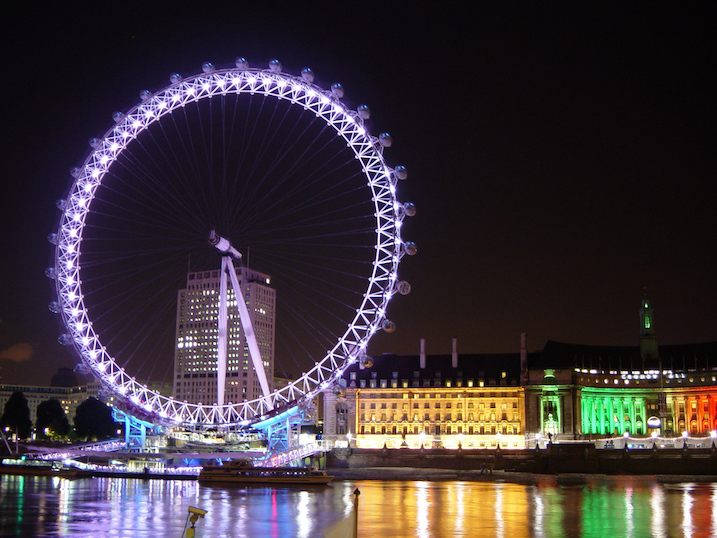
\includegraphics[width=\paperwidth]{London_Eye_-_panoramio_(7)}}
\usepackage{tikz}
\usetikzlibrary{calc}
\usepackage{decorule}

\definecolor{col1}{HTML}{f8a909}
\definecolor{col2}{HTML}{cf122d}
\definecolor{col3}{HTML}{ab378c}
\definecolor{col4}{HTML}{412884}
\definecolor{col5}{HTML}{195da9}
\definecolor{col6}{HTML}{62a830}
\definecolor{col7}{HTML}{ec6728}

\newcounter{maxframe}
\setcounter{maxframe}{800}

\makeatletter
\newcommand*{\slideinframe}{\number\beamer@slideinframe}
\makeatother

\begin{document}
	
\begin{frame}
  \begin{tikzpicture}[remember picture, overlay, font=\sffamily\color{white}]
%    \draw[green,ultra thick] (3,-0.4) circle [radius=2.9];
    
    \foreach \x in {0}{
      \begin{scope}[circle,draw=white,thick,minimum width=3em]
        \node<+>[fill=col1] (B1) at ($(3,-0.4)+(\x+90+0*360/7:2.9)$) {s}; 
        \node<.>[fill=col2] (B2) at ($(3,-0.4)+(\x+90+1*360/7:2.9)$) {kg}; 
        \node<.>[fill=col3] (B3) at ($(3,-0.4)+(\x+90+2*360/7:2.9)$) {mol}; 
        \node<.>[fill=col4] (B4) at ($(3,-0.4)+(\x+90+3*360/7:2.9)$) {cd}; 
        \node<.>[fill=col5] (B5) at ($(3,-0.4)+(\x+90+4*360/7:2.9)$) {K}; 
        \node<.>[fill=col6] (B6) at ($(3,-0.4)+(\x+90+5*360/7:2.9)$) {A}; 
        \node<.>[fill=col7] (B7) at ($(3,-0.4)+(\x+90+6*360/7:2.9)$) {m};   
        \foreach \y in {1,...,7}{
          \draw[white,thick] (B\y) -- (3,-0.4);
        }                
      \end{scope}
    }  
    
 		\node at (15-20*\slideinframe/\themaxframe,-3.5) {
\includegraphics[width=3cm]{joseph}};
    
    \node[white,font=\tiny,text width=\paperwidth,align=center,anchor=south] at (current page.south) {Image source: \url{https://commons.wikimedia.org/wiki/File:London_Eye_-_panoramio_(7).jpg}\linebreak
    Music: \url{https://www.youtube.com/watch?v=h6vca9PnlyI}};
    \fill[black,opacity=0.7] (current page.south east) rectangle (current page.north west);
    \node[text width=.8\textwidth,align=center,font=\Large\color{white}] at (current page.center) { To celebrate all the new features \linebreak and bug fixes of \texttt{siunitx}\bigskip \linebreak \decorule\bigskip \linebreak Thank you @Joseph!};
  \end{tikzpicture}
  \pause[100]
\end{frame}	  
  
\begin{frame}
  \begin{tikzpicture}[remember picture, overlay, font=\sffamily\color{white}]
%    \draw[green,ultra thick] (3,-0.4) circle [radius=2.9];
    
    \foreach \x in {0,-1,...,-\themaxframe}{
      \begin{scope}[circle,draw=white,thick,minimum width=3em]
        \node<+>[fill=col1] (B1) at ($(3,-0.4)+(\x+90+0*360/7:2.9)$) {s}; 
        \node<.>[fill=col2] (B2) at ($(3,-0.4)+(\x+90+1*360/7:2.9)$) {kg}; 
        \node<.>[fill=col3] (B3) at ($(3,-0.4)+(\x+90+2*360/7:2.9)$) {mol}; 
        \node<.>[fill=col4] (B4) at ($(3,-0.4)+(\x+90+3*360/7:2.9)$) {cd}; 
        \node<.>[fill=col5] (B5) at ($(3,-0.4)+(\x+90+4*360/7:2.9)$) {K}; 
        \node<.>[fill=col6] (B6) at ($(3,-0.4)+(\x+90+5*360/7:2.9)$) {A}; 
        \node<.>[fill=col7] (B7) at ($(3,-0.4)+(\x+90+6*360/7:2.9)$) {m};   
        \foreach \y in {1,...,7}{
          \draw[white,thick] (B\y) -- (3,-0.4);
        }        
      \end{scope}
    }  
    
 		\node at (15-20*\slideinframe/\themaxframe,-3.5) {
\includegraphics[width=3cm]{joseph}};
    
    \node[white,font=\tiny,text width=\paperwidth,align=center,anchor=south] at (current page.south) {Image source: \url{https://commons.wikimedia.org/wiki/File:London_Eye_-_panoramio_(7).jpg}\linebreak
    Music: \url{https://www.youtube.com/watch?v=h6vca9PnlyI}};
  \end{tikzpicture}
\end{frame}	
	
\end{document}